\question[5] Considera los dos triángulos que se muestran abajo en la Figura \ref{fig:20230323155215} (los triángulos no están dibujados a escala).

\begin{figure}[H]
    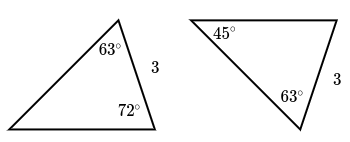
\includegraphics[width=0.5\linewidth]{../images/20230323155215}
    \caption{}
    \label{fig:20230323155215}
\end{figure}

\textbf{¿Los dos triángulos son congruentes?}
\emph{Escoge 1 respuesta:}

\begin{choices}
    \CorrectChoice Sí.
    \choice No.
    \choice No hay suficiente información para decidir.
\end{choices}

\begin{solutionbox}{5cm}
    Dos triángulos son congruentes si tienen la misma forma y tamaño. En otras palabras, dos triángulos son congruentes si todos los lados y ángulos correspondientes son congruentes.
    Sin embargo, no necesitamos mostrar la congruencia de todos los lados y ángulos correspondientes para demostrar que dos triángulos son congruentes. Los criterios de congruencia (LLL, LAL, ALA) y el teorema AAL son atajos útiles para determinar congruencia de triángulos.

    En este caso, nos dan un lado y dos ángulos en cada triángulo.
    Puesto que la suma de las medidas de los ángulos de un triángulo es 180$^\circ$, podemos encontrar el ángulo restante en cada triángulo.

    \begin{figure}[H]
        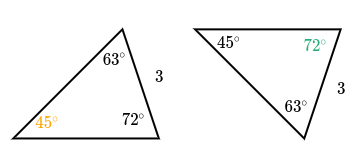
\includegraphics[width=0.45\textwidth]{../images/20230323155725}
        \caption{}
        \label{fig:20230323155725}
    \end{figure}

    Ahora observa que dos ángulos y el lado entre ellos en un triángulo son congruentes a dos ángulos y el lado entre ellos de otro triángulo.

    \begin{figure}[H]
        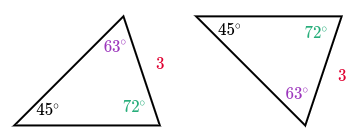
\includegraphics[width=0.45\textwidth]{../images/20230323155732}
        \caption{}
        \label{fig:20230323155732}
    \end{figure}

    Por lo tanto, los triángulos son congruentes por el criterio ALA.
    Sí, los triángulos son congruentes.
\end{solutionbox}